\section{The quasiparticle number model}
\label{sec:theory.qpnumber}

In this section I discuss the steady-state and dynamical behavior of the quasiparticle system using only the density of quasiparticles
$\qpdensity = \braket{\responseqpoccupancy_{\qpdensity}}{\qpoccupancy}$ instead of the function $\qpoccupancy(\energy)$.
The key results are the rate equation for the quasiparticle density (Equation~\ref{eqn:rate_qpdensity}) and its solutions in steady-state (Equation~\ref{eqn:ssqpdensity}) and for time-dependent perturbations (Equation~\ref{eqn:delta_qpdensity_time}).
A new phenomenological quantity emerges: the quasiparticle relaxation time $\qprelaxationtime$, which describes the decay of small perturbations to the density.

\begin{figure}[htb]
\centering
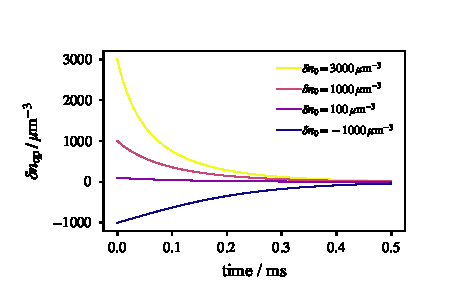
\includegraphics[width=\textwidth]{theory/delta_qpdensity_versus_time.pdf}
\caption
[The decay of perturbations to the quasiparticle density versus time.]
{The decay of perturbations to the quasiparticle density versus time.
The steady-state density is
$\ssqpdensity = \SI{1000}{\micro\meter^{-3}}$,
the effective recombination constant is
$\qprecombinationeff = \SI{3.9}{\micro\meter^{3}.s^{-1}}$
using fiducial values for aluminum with a phonon trapping factor
$\phonontrapping = 2$,
and the single-quasiparticle decay constant $\qpsingledecay$ is zero.
The resulting quasiparticle relaxation time is
$\qprelaxationtime = \SI{127}{\micro\second}$.
Large positive perturbations to the steady-state density can be caused by high-energy photons or other energetic particles.
Large negative perturbations are not expected to occur normally, but they could be created by an abrupt increase in a constant level of illumination.
There is a significant difference in behavior of the two solutions with initial conditions of opposite sign.
Because the sign of the quadratic term in Equation~\ref{eqn:rate_delta_qpdensity} is always negative, large negative perturbations initially relax more slowly to the steady-state value than large positive perturbations, and this distinction vanishes when the perturbation is small.
\todo[inline]{Recreate this $\qpdensity(\time)$ figure with a smaller steady-state density.}
}
\label{fig:delta_qpdensity_versus_time}
\end{figure}

Using Equation~\ref{eqn:rate_qprecombination} (with phonon trapping included) and Equation~\ref{eqn:rate_qpsingledecay}, the rate equation for the evolution of a homogeneous quasiparticle density is
\begin{equation}
\dv{\qpdensity(\time)}{\time}
  =
  \rate_\generation(\time)
  - \rate_\qprecombinationeff(\time)
  - \rate_\qpsingledecay(\time)
  =
  \rate_\generation(\time)
  -\qprecombinationeff \qpdensity(\time)^2
  -\qpsingledecay \qpdensity(\time).
\label{eqn:rate_qpdensity}
\end{equation}
The first term is the total generation rate per unit volume.
The second and third terms are, respectively, the decay rates per unit volume due to quasiparticle recombination in pairs with phonon emission (including phonon trapping) and due to single-quasiparticle decay.
See Appendix~\ref{chp:connections} for discussion of similar rate equations.


\subsection{Steady-state}
\label{sec:theory.qpnumber.steady-state}

For a constant generation rate
$\rate_\generation(\time) = \ssrate_\generation$,
the time derivative is zero and solving the quadratic equation
\begin{equation}
0
  =
  \ssrate_\generation
  - \qprecombinationeff \ssqpdensity^2
  - \qpsingledecay \ssqpdensity
\label{eqn:ssrate_qpdensity}
\end{equation}
gives the steady-state quasiparticle density
\begin{equation}
\ssqpdensity
  =
  \left[ \left(\frac{\qpsingledecay}{2 \qprecombinationeff}\right)^2
  + \frac{\ssrate_\generation}{\qprecombinationeff} \right]^{1/2}
  - \frac{\qpsingledecay}{2 \qprecombinationeff}.
\label{eqn:ssqpdensity}
\end{equation}
When single-quasiparticle decay is negligible, as we expect to be the case in an illuminated KID, the steady-state density is simply
$
\ssqpdensity
  =
  \left( \ssrate_\generation / \qprecombinationeff \right)^{1/2}.
$
This square-root behavior causes the detector response to be inherently nonlinear for large signals.

\subsection{Dynamics}
\label{sec:theory.qpnumber.dynamics}

To understand the behavior of perturbations around the steady-state density, it is convenient to rewrite Equation~\ref{eqn:rate_qpdensity} in terms of 
$\delta \qpdensity(\time) = \qpdensity(\time) - \ssqpdensity$
and
$\delta\rate_\generation(\time) = \rate_\generation(\time) - \ssrate_\generation$.
Using Equation~\ref{eqn:ssrate_qpdensity} to cancel most of the steady-state values gives
\begin{align}
\begin{split}
\dv{\qpdensity(\time)}{\time}
  =
  \dv{\delta\qpdensity(\time)}{\time}
  &=
  \ssrate_\generation + \delta\rate_\generation(\time)
  -
  \qprecombinationeff \left(\ssqpdensity^2 + 2 \ssqpdensity \delta\qpdensity(\time) + \delta\qpdensity(\time)^2 \right)
  - \qpsingledecay \left( \ssqpdensity + \delta\qpdensity(\time) \right) \\
  &=
  \delta \rate_\generation(\time)
  - \qprecombinationeff \delta\qpdensity(\time)^2
  - \left(2 \qprecombinationeff \ssqpdensity + \qpsingledecay \right) \delta\qpdensity(\time), \\
  &\equiv
  \delta \rate_\generation(\time)
  - \qprecombinationeff \delta\qpdensity(\time)^2
  - \qprelaxationtime^{-1} \delta\qpdensity(\time).
\end{split}
\label{eqn:rate_delta_qpdensity}
\end{align}
Here, $\qprelaxationtime$ is the quasiparticle relaxation time, which can be expressed in several useful forms using Equation~\ref{eqn:ssqpdensity}:
\begin{equation}
\qprelaxationtime
  =
  \left( 2 \qprecombinationeff \ssqpdensity + \qpsingledecay \right)^{-1}
  =
  \left( \frac{2 \ssrate_\generation}{\ssqpdensity} - \qpsingledecay \right)^{-1}
  =
  \left( 4 \qprecombinationeff \ssrate_\generation + \qpsingledecay^2 \right)^{-1/2}
  =
  \pdv{\ssqpdensity}{\ssrate_\generation}.
\label{eqn:qprelaxationtime}
\end{equation}
The relaxation time is important both as a probe of the microscopic physics and as a detector parameter to be optimized.
Before discussing it at length, I examine the behavior of solutions to Equation~\ref{eqn:rate_delta_qpdensity} in two different limits that are relevant to detector operation.

First, consider small perturbations $\delta\rate_\generation$ to the generation rate that maintain the density close to the steady-state value.
The quadratic term will be much smaller than the linear term when a perturbation $\delta\qpdensity$ is sufficiently small to satisfy
\begin{equation}
1
  \gg
  \qprecombinationeff \qprelaxationtime |\delta\qpdensity|
  =
  \frac{|\delta\qpdensity|}{2 \ssqpdensity + \qpsingledecay / \qprecombinationeff}.
\end{equation}
Thus, perturbations that are significantly smaller than the steady-state density are always small, and larger perturbations may also be small if single-quasiparticle decay is significant.
Assume that the generation rate may vary around the mean value but that we can neglect the quadratic term.
Since the optical generation rate is proportional to the absorbed power, this situation corresponds to a KID detecting a small, time-varying signal, as in CMB observation.
Defining Fourier transforms of the time-dependent quantities
\begin{equation}
\delta\qpdensity(\time)
  =
  \int_{-\infty}^\infty \dd{\faudio}
  \exp(2 \pi \I \faudio \time) \, \delta\qpdensity(\faudio)
  \qqtext{and}
\delta\rate_\generation(\time)
  =
  \int_{-\infty}^\infty \dd{\faudio}
  \exp(2 \pi \I \faudio \time) \, \delta\rate_\generation(\faudio),
\end{equation}
a Fourier solution to the linearized form of Equation~\ref{eqn:rate_delta_qpdensity} is
\begin{equation}
\delta\qpdensity(\faudio)
  =
  \frac{\qprelaxationtime}{1 + 2 \pi \I \faudio \qprelaxationtime} \delta\rate_\generation(\faudio).
\label{eqn:delta_qpdensity_frequency}
\end{equation}
As expected, the low-frequency limit of this equation equals the derivative of the steady-state density:
\begin{equation}
\lim_{\faudio \rightarrow 0} \frac{\delta\qpdensity(\faudio)}{\delta\rate_\generation(\faudio)}
  =
  \qprelaxationtime
  =
  \pdv{\ssqpdensity}{\ssrate_\generation}.
\end{equation}
The response to small, time-varying signals has single-pole behavior with a cutoff frequency 
$\faudio_\quasiparticle = (2 \pi \qprelaxationtime)^{-1}$.
This indicates that the spectral density of the quasiparticle density (or number) fluctuations has a Lorentzian shape with a bandwidth set by the relaxation time.
\todo[inline]{and this conclusion is derived more rigorously in Appendix~chp:fluctuations}

Second, consider a sudden perturbation $\delta\qpdensity(0)$ that is sufficiently large that we can neglect fluctuations in the generation rate and set
$\delta\rate_\generation = 0$.
This is a reasonable description of a KID that absorbs a high-energy photon or is hit by a cosmic ray, both of which may quickly generate a large number of quasiparticles.
(There is no physical process that is expected to instantly annihilate a large number of quasiparticles.
However, immediately after an abrupt increase in an otherwise constant illumination rate the initial perturbation would be negative, though it must satisfy
$\delta\qpdensity(0) > -\ssqpdensity$.)
In this limit, the solution for $\time > 0$ is 
\begin{equation}
\delta\qpdensity(\time)
  =
  \frac{\delta\qpdensity(0)}
  {1 + [1 + \qprecombinationeff \qprelaxationtime \delta\qpdensity(0)] 
  [\exp(\time / \qprelaxationtime) - 1]}.
\label{eqn:delta_qpdensity_time}
\end{equation}
\todo[inline]{In Appendix ... I derive this solution and discuss some of its implications for the measurement of high-energy photons.}
Even for large perturbations where $\qprecombinationeff \qprelaxationtime \, \delta\qpdensity(0) \gg 1$, after a time of order $\qprelaxationtime$ the system will have recovered to an excess density $\delta\qpdensity \sim (\qprecombinationeff \qprelaxationtime)^{-1} = 2 \ssqpdensity + \qpsingledecay / \qprecombinationeff$.
When a perturbation satisfies
$\qprecombinationeff \qprelaxationtime |\delta\qpdensity(\time)| \ll 1$,
either initially or after some decay, the behavior of the solution at later times is exponential decay to the steady-state value, which is also the solution of the rate equation when the quadratic term is negligible.
This extremely rapid decay from large density perturbations is a major advantage for CMB observation, since such perturbations are likely to render the data useless until the density approaches the steady-state value.

Figure~\ref{fig:mkidarray02_chosen_one_x_fold_fit} shows a fit of Equation~\ref{eqn:delta_qpdensity_time} to time-ordered data from one of the co-planar waveguide KIDs described in Chapter~\ref{chp:multichroic}.
The detector was illuminated by light from an electronic millimeter-wave source described in Section~\ref{sec:sensitivity.measuring} and Appendix~\ref{sec:hardware.mmw_source}.
The data shows the response as the illumination is turned off.
(More of this data set is shown in Figure~\ref{fig:mkidarray02_chosen_one_mmw_decimated_and_folded}.)
The quasiparticle relaxation time given in the legend is extracted from the fit.
It should be possible to measure $\qprecombinationeff$ by combining careful measurements of detector response to thermal quasiparticles with measurements at different illumination levels.

\begin{figure}[htb]
\centering
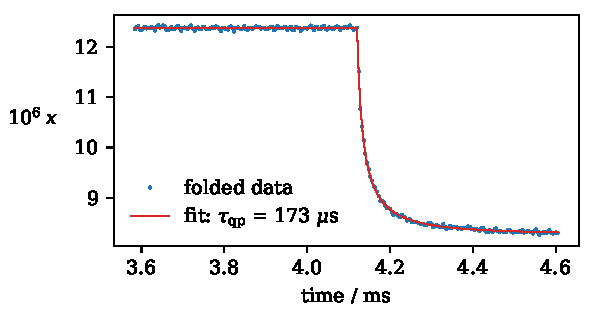
\includegraphics[width=\textwidth]{theory/mkidarray02_chosen_one_x_fold_fit.pdf}
\caption[Time-ordered data showing the detuning response as a millimeter-wave signal is turned off, and a fit.]
{
Time-ordered data showing the detuning response as a millimeter-wave signal is turned off, and a fit to Equation~\ref{eqn:rate_delta_qpdensity} multiplied by a constant.
The quantity plotted on the vertical axis is the response of the detector expressed as a fractional shift in the resonance frequency, discussed in Section~\ref{sec:theory.resonator} below.
}
\label{fig:mkidarray02_chosen_one_x_fold_fit}
\end{figure}


\subsection{The quasiparticle relaxation time}
\label{sec:theory.qpnumber.qprelaxationtime}

From the expression
$\qprelaxationtime
  =
  \left( 4 \qprecombinationeff \ssrate_\generation + \qpsingledecay^2 \right)^{-1/2}$,
we see that the relaxation time depends on all the microscopic creation and annihilation processes:
$\ssrate_\generation$ is the sum of generation rates from all sources,
$\qprecombinationeff = \qprecombination / \phonontrapping$
involves pair recombination modified by phonon trapping, and $\qpsingledecay$ includes all single-quasiparticle decay sources.
The two solutions to the rate equation discussed above illustrate the two common methods for measuring $\qprelaxationtime$ directly.
One method, shown in Figure~\ref{fig:mkidarray02_chosen_one_x_fold_fit}, involves fitting the decay back to steady-state in order to extract the time constant governing the exponential tail of the decay.
Another method involves fitting the roll-off in the spectral density of time-ordered data, which requires the quasiparticle noise to be measurable.
Both of these methods require the quasiparticle bandwidth $\faudio_\quasiparticle$ to be much less than either the bandwidth of the resonator or the bandwidth of the readout system.

The exponential temperature dependence of the thermal generation rate makes it possible to reduce it to very low levels.
At sufficiently low temperatures, some other generation source may dominate, such as readout photons or optical photons leaking into a nominally sealed package.
When the total generation rate becomes constant as the temperature is further reduced, $\qprelaxationtime$ will saturate, or remain constant at some maximum value~\autocite{deVisser2011PRL}.
Alternatively, if some single-quasiparticle decay channel becomes dominant at sufficiently low density, $\qprelaxationtime$ will saturate because the decay rate per quasiparticle is independent of the density.
Merely observing saturation does not allow us to identify its cause.

\todo[inline]{Decide how much of this to include.}
\begin{comment}
In this section I give a quick survey of experimental results regarding quasiparticle behavior at low densities and connect these results to the experimental situation in our laboratory.
The conclusion will be that single-quasiparticle decay is not necessary to explain saturation of the relaxation time in our experiments, and that the relaxation time is instead likely to be limited by optical quasiparticle generation, even when the devices are tested under apparently dark conditions.
I will interpret later results assuming that $\qpsingledecay$, the constant for all single-quasiparticle decay processes, can be set to zero without significant error.

\textcite{Wang2014NatComm} measured the decay of the quasiparticle density over several orders of magnitude in thin-film aluminum qubits and compared the results to the solutions of an equation equivalent to Equation~\ref{eqn:rate_qpdensity}.
By controlling the number of magnetic flux vortices using a magnetic field normal to the film, they were able to control the single-quasiparticle trapping rate.
In a device with many vortices, they observed exponential decay, presumably dominated by single-quasiparticle trapping in vortices, over most of the density range.
However, in a device with few or no vortices, they observed decay curves well-described by only the quadratic pair-recombination term in the rate equation.
The longest relaxation time they measured was \SI{18}{ms} and the background trapping rate observed with no vortices present was small.
\end{comment}

Several studies~\autocite{Baselmans2009AIPC, Barends2011APL, Corcoles2011APL, Barends2011APL, Kreikebaum2016SUST} have shown that ambient radiation from the experimental volume can leak into a sealed metal package, but that the resulting quasiparticle generation can be made negligible by using line filters on the coaxial cables entering the package, coating the inside of the package with an infrared absorbing material, enclosing the package in a metal box with absorbing material on the inside, and sealing the seams in the package with metal tape.
Studies that have fully implemented such enhanced shielding typically measure relaxation times of several \si{ms}~\autocite{Baselmans2009AIPC,deVisser2014NatComm}
in aluminum devices.

\begin{figure}[tb]
\centering
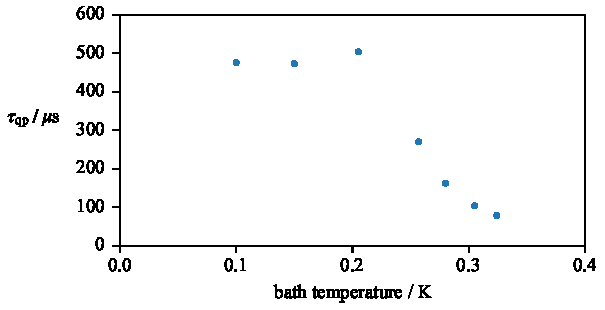
\includegraphics[width=\textwidth]{theory/tau_qp_vs_bath_temperature.pdf}
\caption
[The quasiparticle relaxation time versus bath temperature, showing saturation at low temperature.]
{
The quasiparticle relaxation time versus bath temperature, showing saturation at low temperature.
The device tested was an aluminum lumped-element KID.
Because the resonator bandwidth of these devices was comparable to the quasiparticle bandwidth, I performed these measurements at a frequency corresponding to a higher order resonance.
The relaxation time was extracted by fitting the exponential tail of the decay of the detector response to a pulse from an LED.
This data set was published in \textcite{McCarrick2014RSI}.
}
\label{fig:tau_qp_vs_bath_temperature}
\end{figure}

Figure~\ref{fig:tau_qp_vs_bath_temperature} shows measurements of the quasiparticle relaxation time versus bath temperature.
The device was an aluminum lumped-element KID tested inside a sealed aluminum package (a ``dark'' test) that was enclosed in a copper box containing a chunk of highly absorbent material.
The quasiparticle relaxation time saturates at \SI{0.5}{ms}.
This is the longest time we have observed in any experiment but is less than was achieved in the studies with better shielding.
In other experiments, we have regularly used aluminum or copper tape to seal the seams in packages but have not generally used other shielding.
Thus, even in our dark measurements, saturation is likely to be caused by background quasiparticle generation due to stray light.
In experiments where detectors are tested optically, the detectors are exposed the much higher ambient light level in the experimental volume, which is typically of order \SI{3}{K}.

It may be possible to measure the relaxation time indirectly, using steady-state measurements, but this requires careful interpretation.
Assume that constant power $\power$ excites quasiparticles with average energy close to $\gap$ in a superconductor occupying volume $\volume$.
Then, energy conservation yields
\begin{equation}
\power / \volume
  =
  \ssrate_\generation \gap
  =
  \left( \ssrate_\qprecombinationeff + \ssrate_\qpsingledecay \right) \gap
  =
  \gap \qpdensity / \tau,
\end{equation}
for some time $\tau$.
What is the relationship between $\tau$ and the relaxation time $\qprelaxationtime$?
Using Equation~\ref{eqn:rate_qpdensity}, 
\begin{equation}
\tau^{-1}
  =
  \frac{\ssrate_\qprecombinationeff + \ssrate_\qpsingledecay}{\ssqpdensity}
  =
  \qprecombinationeff \ssqpdensity + \qpsingledecay.
\end{equation}
Comparing this to
$\qprelaxationtime^{-1} = 2 \qprecombinationeff \ssqpdensity + \qpsingledecay$,
we see that the relationship between these times depends on the balance between pair recombination and single-quasiparticle decay.
In particular, the equation
$\power = \gap \ssqpdensity / \qprelaxationtime$
is correct \textit{only} when pair recombination is negligible.
In the opposite limit, where single-quasiparticle decay is negligible, the relationship is $\qprelaxationtime = \tau / 2$.
The factor of two arises from linearization of the quadratic recombination term.

This illustrates the confusing point that there are several ``lifetimes'' associated with the quasiparticle system.
The pair-recombination lifetime $\qprecombinationtime$ is not directly accessible to typical experiments using superconducting resonators.
Instead, these measure $\phonontrapping \qprecombinationtime$, the \textit{effective} lifetime of a single quasiparticle, extended due to the phonon trapping effect discussed in Section~\ref{sec:theory.quasiparticle.phonons}.
If single-quasiparticle decay is negligible than this latter quantity equals $\tau$ in the energy conservation equation above, and it could be measured in steady-state experiments.
The relaxation time $\qprelaxationtime$ is the quantity extracted from dynamic experiments that measure pulse decay or quasiparticle bandwidth.
